\documentclass[border=0.8ex,svgnames,tikz]{standalone}
\usepackage{amsmath,mathtools}
\usepackage{fontspec}
\setmainfont{Source Serif 4}
\setsansfont{Source Sans 3}
\setmonofont{Source Code Pro}

\usetikzlibrary{calc,chains,shapes.multipart}

\begin{document}
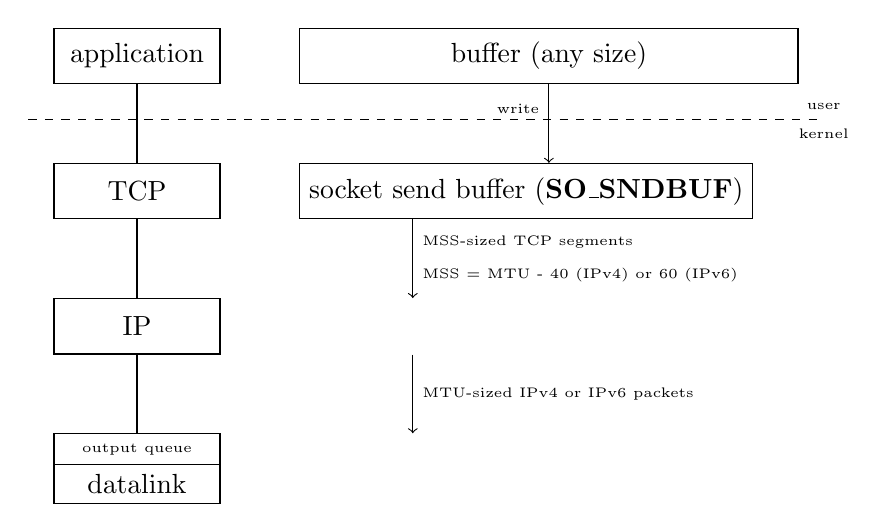
\begin{tikzpicture}
    \begin{scope}[
    protochain node/.style={
      draw,
      on chain,
      align=center,
      minimum width=6em,
      minimum height=2em,
    },
    start chain=going below,
    every on chain/.style={join},
    ]
    \node[protochain node] (application) {application};
    \node[protochain node] (transport)   {TCP};
    \node[protochain node] (internet)    {IP};
    \node[protochain node,
          rectangle split,
          rectangle split parts=2,
          rectangle split ignore empty parts,
          rectangle split part align=base,] (link) {{\tiny output queue}
            \nodepart{two} datalink};
  \end{scope}
  \begin{scope}[
    buffer node/.style={
      draw,
      on chain,
      anchor=north west,
      minimum width=15em,
      minimum height=2em,
    },
    buffer coor/.style={
      on chain,
    },
    start chain=going {below=of \tikzchainprevious.south west},
    every path/.style={draw,->},
    ]
    \node[buffer node,minimum width=18em,right=1 of application] (user-buffer)   {buffer (any size)};
    \node[buffer node] (kernel-buffer) {socket send buffer (\textbf{SO\_SNDBUF})};
    \coordinate[buffer coor] (internet-buffer);
    \coordinate[buffer coor] (link-buffer);
    \path[draw,->] (user-buffer.south) -- node[align=right,above left]{\tiny write}
    ++($(kernel-buffer.north west)-(user-buffer.south west)$);
    \path[draw,->] ($(kernel-buffer.south west)!0.5!(kernel-buffer.south)$) --
    node[align=left,right]{{\tiny MSS-sized TCP segments}\\{\tiny
        MSS = MTU - 40 (IPv4) or 60 (IPv6)}}
    ++($(internet-buffer)-(kernel-buffer.south west)$) coordinate(temp-coor);
    \path[draw,->] (temp-coor) ++($(kernel-buffer.south)-(kernel-buffer.north)$)
    -- node[align=left,right]{\tiny MTU-sized IPv4 or IPv6 packets} ++($(link-buffer)-(internet-buffer)$);
  \end{scope}
  \begin{scope}[every node/.style={draw=none,anchor=east,font=\tiny}]
   \coordinate (API-line-begin) at ($(application.south west)-(+0.32,+0.45)$);
    \coordinate (API-line-end)   at ($(user-buffer.south east)+(+0.32,-0.45)$);
    \path[draw,dashed] (API-line-begin) -- (API-line-end)
      node[below]{kernel} node[above]{user};
  \end{scope}
\end{tikzpicture}
\end{document}
